\subsection{Triangles}
변 길이 $a,b,c$; $p=\frac{a+b+c}{2}$

넓이 $A=\sqrt{p(p-a)(p-b)(p-c)}$

외접원 반지름 $R=\frac{abc}{4A}$

내접원 반지름 $r=\frac{A}{p}$

중선 길이 $m_a = \frac{1}{2} \sqrt{2b^2+2c^2-a^2}$

각 이등분선 길이 $s_a = \sqrt{bc(1-(\frac{a}{b+c})^2)}$

사인 법칙 $\frac{\sin A}{a}=\frac{1}{2R}$

코사인 법칙 $a^2=b^2+c^2-2bc \cos A$

탄젠트 법칙 $\frac{a+b}{a-b} = \frac{\tan (A+B)/2}{\tan (A-B)/2}$

중심 좌표 $(\frac{\alpha x_a + \beta x_b + \gamma x_c}{\alpha+\beta+\gamma}, \frac{\alpha y_a + \beta y_b + \gamma y_c}{\alpha+\beta+\gamma})$ where

\begin{tabular}{|c||c|c|c||c|}
    \hline
    이름 & $\alpha$ & $\beta$ & $\gamma$ & \\
    \hline
    외심 & $a^2 \mathcal{A}$ & $b^2 \mathcal{B}$ & $c^2 \mathcal{C}$ & $\mathcal{A} = b^2+c^2-a^2$\\
    내심 & $a$ & $b$ & $c$ & $\mathcal{B} = a^2+c^2-b^2$ \\
    무게중심 & 1 & 1 & 1 & $\mathcal{C} = a^2+b^2-c^2$\\
    수심 & $\mathcal{BC}$ & $\mathcal{AC}$ & $\mathcal{AB}$ & \\
    방심($A$) & $-a$ & $b$ & $c$ & \\
    \hline
\end{tabular}

\subsection{Series And Calculus}

\begin{tabular}{c|c}
    \hline
    $(\arcsin x)' = \frac{1}{\sqrt{1-x^2}}$ & $(\arccos x)' = -\frac{1}{\sqrt{1-x^2}}$ \\
    $(\tan x)' = 1 + \tan^2 x$ & $(\arctan x)' = \frac{1}{1+x^2}$ \\
    $\int{\tan ax} = -\frac{\ln |\cos ax|}{a}$ & $\int{x \sin ax} = (\sin ax - ax \cos ax)/a^2$ \\
    \hline
\end{tabular}

\begin{displaymath}
    \ointctrclockwise _C (Ldx+Mdy) = \iint _D (\frac{\partial M}{\partial x} - \frac{\partial L}{\partial y})dxdy
\end{displaymath}

where $C$ is positively oriented, piecewise smooth, simple, closed; $D$ is the region inside $C$; $L$ and $M$ have continuous partial derivatives in $D$.

\subsection{Theorems}

\textbf{Kirchhoff's theorem}: The number of spanning trees equals any cofactor of its Laplacian matrix.

\textbf{Dilworth's theorem}: In a finite partially ordered set, maximum antichain equals minimum chain cover.

\textbf{Euler's theorem 1}: For coprime $a$ and $n$, $a^{\phi(n)} \equiv 1$ (mod $n$).

\textbf{Euler's theorem 2}: Generally, $a^n \equiv a^{n-\phi(n)}$ (mod $n$).

\textbf{Euler's theorem 3}: For $m \geq \log_2 n$, $a^m \equiv a^{m\%\phi(n) + \phi(n)}$ (mod $n$).

\textbf{Konig's theorem}: In a bipartite graph, maximum matching equals minimum vertex cover.

\textbf{Hall's theorem}: A bipartite graph with partition $(A,B)$ has a perfect matching iff for $X \subseteq A$, $|X| \leq |N_G(X)|$.

\textbf{Pick's theorem}: $A = i+\frac{b}{2}-1$.

\textbf{Burnside's lemma}: Let a finite group $G$ act on a set $X$, then $|X/G| = \frac{1}{|G|}\sum_{g \in G}|X^g|$.

\subsection{Combinatorics}

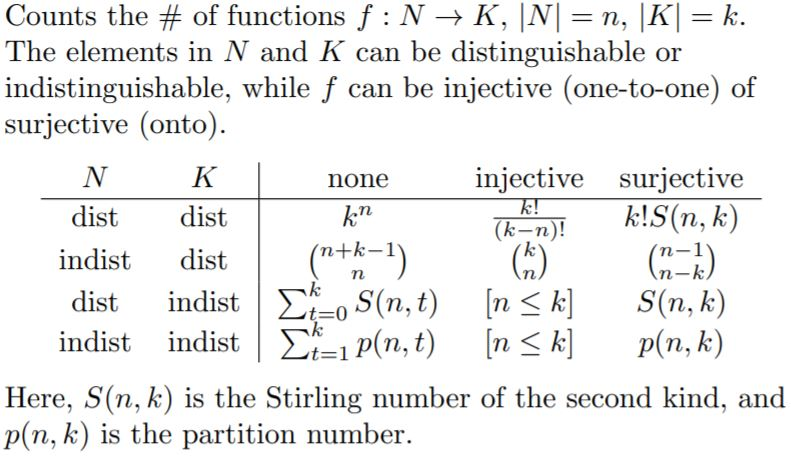
\includegraphics[width=10cm]{twelvefold.JPG}

Derangement: $D(n) = (n-1)(D(n-1)+D(n-2))$

Sgn Stirling 1: $S_1(n,k) = (n-1)S_1(n-1,k) + S_1(n-1,k-1)$

Unsgn Stirling 1: $C_1(n,k) = (n-1)c_1(n-1,k) + C_1(n-1,k-1)$

Stirling 2: $S_2(n,k) = kS_2(n-1,k) + S_2(n-1,k-1)$

Stirling 2: $S_2(n,k) = \frac{1}{k!} \sum_{j=0}{k} (-1)^{k-j} \binom{k}{j} j^n$

Partition: $p(n,k) = p(n-1,k-1) + p(n-k,k)$

Partition: $p(n) = \sum (-1)^k p(n-k(3k-1)/2)$

Bell: $B(n) = \sum_{k=1}^{n} \binom{n-1}{k-1}B(n-k)$

Catalan: $C_n = \frac{1}{n+1}\binom{2n}{n}$

Catalan: $C_n = \binom{2n}{n} - \binom{2n}{n+1}$

Catalan: $C_n = \frac{(2n)!}{(n+1)!n!}$

Catalan: $C_n = \sum C_i C_{n-i}$

\subsection{Composite and Prime}
$n \leq 1,000,000$ 약수 최대 240개 (720,720)

$n \leq 1,000,000,000$ 최대 1,344개 (735,134,400)

up to 10,000: 소수 1,229개 (9,973)

up to 100,000: 소수 9,592개 (99,991)

up to 1,000,000: 소수 78,498개 (999,983)

up to 1,000,000,000: 소수 50,847,534개 (999,999,937)

10,007; 10,009; 10,111; 31,567; 70,001; 1,000,003; 1,000,033

99,999,989; 999,999,937; 1,000,000,007; 9,999,999,967

$998244353 = 119 \times 2^{23} + 1$, primitive 3

$985661441 = 235 \times 2^{22} + 1$, primitive 3

$1012924417 = 483 \times 2^{21} + 1$, primitive 5

\subsection{Pythagorean Triples}
The Pythagorean triples are uniquely generated by $a=k(m^2-n^2)$, $b=k(2mn)$, $c=k(m^2+n^2)$ where $m>n>0, k>0, gcd(m,n)=1$, and either $m$ or $n$ is even.